% $Header: /data/cvsroot/Courses/OnlineLearning/talks/talk3/talk3.tex,v 1.2 2006/01/18 02:26:18 yfreund Exp $

%\documentclass{beamer}
\documentclass[handout]{beamer}
% This file is a solution template for:

% - Giving a talk on some subject.
% - The talk is between 15min and 45min long.
% - Style is ornate.

% Copyright 2004 by Till Tantau <tantau@users.sourceforge.net>.
%
% In principle, this file can be redistributed and/or modified under
% the terms of the GNU Public License, version 2.
%
% However, this file is supposed to be a template to be modified
% for your own needs. For this reason, if you use this file as a
% template and not specifically distribute it as part of a another
% package/program, I grant the extra permission to freely copy and
% modify this file as you see fit and even to delete this copyright
% notice. 


\mode<presentation>
{
  \usetheme{Montpellier}

  %\setbeamercovered{transparent}
  % or whatever (possibly just delete it)
}

\usepackage{xmpmulti} % package that defines \multiinclude

\usepackage[english]{babel}

\usepackage[latin1]{inputenc}

\usepackage{times}
\usepackage[T1]{fontenc}
% Or whatever. Note that the encoding and the font should match. If T1
% does not look nice, try deleting the line with the fontenc.

\title[log loss] % (optional, use only with long paper titles)
{Lossless compression \\ and \\ cumulative log loss}

\author[Freund] % (optional, use only with lots of authors)
{Yoav Freund}
% - Give the names in the same order as the appear in the paper.
% - Use the \inst{?} command only if the authors have different
%   affiliation.

\institute[Universities of Somewhere and Elsewhere] % (optional, but mostly needed)

\subject{Machine Learning}
% This is only inserted into the PDF information catalog. Can be left
% out. 

% If you have a file called "university-logo-filename.xxx", where xxx
% is a graphic format that can be processed by latex or pdflatex,
% resp., then you can add a logo as follows:

% \pgfdeclareimage[height=0.5cm]{university-logo}{university-logo-filename}
% \logo{\pgfuseimage{university-logo}}



% Delete this, if you do not want the table of contents to pop up at
% the beginning of each subsection:
%% \AtBeginSubsection[]
%% {
%%   \begin{frame}<beamer>
%%     \frametitle{Outline}
%%     \tableofcontents[currentsection,currentsubsection]
%%   \end{frame}
%% }


% If you wish to uncover everything in a step-wise fashion, uncomment
% the following command: 

\beamerdefaultoverlayspecification{<+->}

\newcommand{\newmcommand}[2]{\newcommand{#1}{{\ifmmode {#2}\else\mbox{${#2}$}\fi}}}
\newcommand{\renewmcommand}[2]{\renewcommand{#1}{{\ifmmode {#2}\else\mbox{${#2}$}\fi}}}
\newcommand{\newmcommandi}[2]{\newcommand{#1}[1]{{\ifmmode {#2}\else\mbox{${#2}$}\fi}}}
\newcommand{\newmcommandii}[2]{\newcommand{#1}[2]{{\ifmmode {#2}\else\mbox{${#2}$}\fi}}}
\newcommand{\newmcommandiii}[2]{\newcommand{#1}[3]{{\ifmmode {#2}\else\mbox{${#2}$}\fi}}}

\newcommand{\algfnt}{\bf}

\newmcommand{\ouralg}{{\mbox{\algfnt Hedge}({\eta})}}

\newmcommand{\iter}{T}

\newfont{\cmmib}{cmmib10}
\newcommand{\boldell}{{\mbox{\cmmib \symbol{'140}}}}


\newmcommandi{\costvec}{{\boldell}^{#1}}
\newmcommandii{\cost}{{\ell}^{#1}_{#2}}

\newmcommandi{\rd}{\tilde{#1}}

\newmcommandi{\distvec}{{\bf p}^{#1}}
\newmcommandi{\rddistvec}{\rd{\bf p}^{#1}}
\newmcommandii{\dist}{{p}^{#1}_{#2}}
\newmcommandii{\rddist}{\rd{p}^{#1}_{#2}}

\newmcommandi{\bdistvec}{{\bf q}^{#1}}
\newmcommandii{\bdist}{{q}^{#1}_{#2}}

\newmcommandi{\wtvec}{{\bf w}^{#1}}
\newmcommandi{\rdwtvec}{\rd{\bf w}^{#1}}
\newmcommandii{\wt}{{w}^{#1}_{#2}}
\newmcommandii{\rdwt}{\rd{w}^{#1}_{#2}}


\newcommand{\Nweight}[2]{V_{#1}^{#2}}	%the normalized weight
\newcommand{\dweight}[2]{w^{#2}(#1)} % initial density measure
\newcommand{\TEloss}[1]{L_{#1}}	%total loss of expert i
\newcommand{\BEloss}{L_{\min}}	%total loss of the best expert
\newcommand{\TAloss}{L_A}	%total loss of algorithm
\newcommand{\weight}[2]{W_{#1}^{#2}} % weight assigned to expert
\newcommand{\btheta}{\hat{\theta}}

\newcommand{\R}[1]{{\color{red}{#1}}}
\newcommand{\B}[1]{{\color{blue}{#1}}}
\newcommand{\RM}[1]{{\color{red}{$#1$}}}


%BANDITS
\newcommand{\Aplay}{{\bf Hedge}}
\newcommand{\Aest}{{\bf Exp3}}
\newcommand{\Aesthp}{{\bf Exp3.P}}
\newcommand{\Aestg}{{\bf Exp3.P.1}}
\newcommand{\Aests}{{\bf Exp3.S}}
\newcommand{\Aessg}{{\bf Exp3.S.1}}
\newcommand{\Astrat}{{\bf Exp4}}
\newcommand{\Abound}{{\bf Exp3.1}}
\newcommand{\Gbest}{G_{\rm max}}

\newcommand{\defeq}{\stackrel{\rm def}{=}}
\newcommand{\compl}{\mbox{\sc h}}
\newcommand{\theset}[2]{\{ {#1} \,:\, {#2} \}}

\newmcommandii{\stratv}{\mbox{\boldmath $\xi$}^{#1}({#2})}

%Games paper
\newmcommand{\M}{\bf M}
\newmcommand{\dM}{\M'}
\newmcommand{\Row}{\bf R}
\newmcommand{\dRow}{\R'}
\newmcommand{\C}{\bf C}
\newmcommand{\dC}{\C'}
\newmcommand{\D}{D}
\renewmcommand{\P}{\bf P}
\newmcommand{\Q}{\bf Q}
\newmcommand{\Dt}{\D_t}
\newmcommand{\Pt}{\P_t}
\newmcommand{\Qt}{\Q_t}
\newmcommand{\Pstar}{\P^*}	% the min/max optimal mixed strategy
\newmcommand{\Pref}{\tilde{\P}}	% a reference mixed strategy (not
				% necessarily min/max)
\newmcommand{\Qstar}{\Q^*}
\newmcommand{\Pa}{\overline{\P}}
\newmcommand{\Qa}{\overline{\Q}}
\newmcommand{\Qh}{\hat{\Q}}
\newmcommandi{\trans}{{#1}^{\rm T}}
\newmcommand{\mhx}{\M(h,x)}
\newmcommand{\mxh}{\dM(x,h)}
\newmcommand{\mpq}{\M(\P,\Q)}
\newmcommand{\mpsq}{\M(\Pstar,\Q)}
\newmcommand{\mpsqt}{\M(\Pstar,\Qt)}
\newmcommand{\mptqt}{\M(\Pt,\Qt)}
\newmcommand{\mptt}{\M(\Pt,t)}
\newmcommand{\mptq}{\M(\Pt,\Q)}
\newmcommand{\mpqt}{\M(\P,\Qt)}
\newcommand{\minp}{\min_{\P}}
\newcommand{\maxq}{\max_{\Q}}
\newcommand{\RE}[2]{{\rm RE}\left( {#1} \; \parallel \; {#2} \right) }

\newmcommand{\sumt}{\sum_{t=1}^T}
\newmcommand{\sumin}{\sum_{i=1}^n}
\newmcommand{\delt}{\Delta_{T,n}}
\newcommand{\nextline}{\vspace{0.2cm}\\}   % a little space for equation arrays

\newcommand{\lwalg}{\mbox{\rm MW}}
\newcommand{\lwalgvar}{\mbox{\rm vMW}}

%%
\newcommand{\E}{\mbox{\rm\bf E}}
\newcommand{\p}[2]{p_{#1}(#2)}
\newcommand{\q}[2]{q_{#1}(#2)}
\newcommand{\x}[2]{x_{#1}({#2})}
\newmcommand{\bx}{\mbox{\boldmath$x$}}
\newmcommandi{\xv}{\bx({#1})}
\newmcommand{\xvt}{\xv{t}}
%\newcommand{\w}[2]{w_{#1}({#2})} replaced by \wt, but remember to switch order of parameters i and t
\renewcommand{\i}[1]{i_{#1}}
\newcommand{\hx}[2]{\hat{x}_{#1}(#2)}
\newcommand{\hxit}{\hx{\i{t}}{t}}
\newcommand{\pit}{\p{\i{t}}{t}}
\newcommand{\xit}{\x{\i{t}}{t}}
\newcommand{\expb}[1]{\exp\left(#1\right)}

\newcommand{\vp}{{\mathbf p}}
\newcommand{\vu}{{\mathbf u}}
\newcommand{\vv}{{\mathbf v}}
\newcommand{\vx}{{\mathbf x}}
\newcommand{\vy}{{\mathbf y}}

\newcommand{\HedgeLoss}{L_{\mbox{\footnotesize Hedge}}}

\newcommand{\W}{\vec{W}}
\newcommand{\V}{\vec{V}}
\newcommand{\X}{\vec{X}}
\newcommand{\vb}{\vec{b}}
%\newcommand{\loss}{\vec{\ell}}
\newcommand{\loss}{L}
%\newcommand{\elloss}[2]{\ell_{#1}^{#2}} %loss of expert i at time t
\newcommand{\elloss}[2]{\ell_{#2}\left( #1 \right)} %loss of expert i at time t
\newcommand{\w}[1]{\makebox[12pt]{{#1}}}
\newcommand{\Rps}{\mbox{\tt R}}
\newcommand{\rPs}{\mbox{\tt P}}
\newcommand{\rpS}{\mbox{\tt S}}
\newcommand{\rpstie}{\w{$\frac{1}{2}$}}
\newcommand{\rpswin}{\w{$0$}}
\newcommand{\rpsloss}{\w{$1$}}

\newmcommand{\decspace}{\Delta}
\newmcommand{\decsym}{\delta}
\newmcommandi{\dec}{\decsym^{#1}}
\newmcommand{\decdistsym}{\cal D}
\newmcommandi{\decdist}{{\decdistsym}^{#1}}

\newmcommand{\simpdistspace}{{\bf \cal S}}
\newmcommand{\domset}{{\rm dom}(\decdistsym)}

\newmcommand{\expdistsym}{{\cal E}}
\newmcommandii{\expdist}{{\expdistsym}^{#1}_{#2}}
\newmcommand{\expdecsym}{{\varepsilon}}
\newmcommandii{\expdec}{\expdecsym^{#1}_{#2}}

\newmcommand{\outspace}{\Omega}
\newmcommand{\outsym}{\omega}
\newmcommandi{\out}{\outsym^{#1}}

%\newmcommandii{\Dkl}{D_{\mbox{kl}}\paren{#1||#2}}
\newmcommandii{\Dkl}{{\rm {KL}}\paren{{#1}\;||\;{#2}}}

\newmcommandi{\sumwts}{\sum_{i=1}^N \wt{#1}{i}}

\newmcommand{\lossalg}{L_A}
\newmcommand{\lossouralg}{{L_{\mbox{\scriptsize\algfnt Hedge}(\eta)}}}
\newmcommand{\lossS}{{L_{\mbox{\scriptsize\algfnt S}}}}
\newmcommandi{\lossi}{L_{#1}}
\newmcommandii{\lossit}{L_{#1}^{#2}}

\newmcommandi{\upbnd}{\tilde{#1}}

\newcommand{\angles}[1]{{\left\langle {#1} \right\rangle}}
\newcommand{\paren}[1]{{\left( {#1} \right)}}
\newcommand{\brac}[1]{{\left[ {#1} \right]}}
\newcommand{\braces}[1]{{\left\{ {#1} \right\}}}

\newcommand{\abs}[1]{{\left| {#1} \right|}}
\newcommand{\ceiling}[1]{{\left\lceil {#1} \right\rceil}}

\newfont{\msym}{msbm10}
\newcommand{\real}{\mbox{\msym R}}

\newmcommand{\updatefcn}{U_\eta}

%% \newtheorem{theorem}{Theorem}	
%% \newtheorem{lemma}[theorem]{Lemma}
%% \newtheorem{corollary}[theorem]{Corollary}
%% \newtheorem{definition}{Definition}

%\newcommand{\proof}{\noindent{\bf Proof:} }
%\newcommand{\example}[1]{{\em Example #1.} }
%\newcommand{\qed}{\rule{0.7em}{0.7em}}

\newcommand{\WeakAlg}{\mbox{\algfnt WeakLearn}}
\newcommand{\Boost}{\mbox{\algfnt AdaBoost}}
\newcommand{\EX}{\mbox{\bf EX}}
\newmcommand{\hf}{h_{{f}}}
\newmcommand{\rdhf}{\rd{h}_{{f}}}
\newmcommand{\hfT}{h^T_{{f}}}
\newmcommand{\ranh}{{b}}

\newmcommand{\conclass}{{\cal C}}

\newmcommand{\badvec}{{\bf b}}
\newmcommandi{\bad}{{b}_{#1}}

%%%%%%%% New commands defined for the game-playing paper

\newmcommand{\hedge}{\algfnt Hedge}
\newmcommand{\play}{\algfnt Play}
\newmcommandi{\Glossvec}{{\bg y}^{#1}}
\newmcommandii{\Gloss}{{y}^{#1}_{#2}}
%\newmcommandi{\action}{{I}_{#1}}
\newmcommandi{\Gdistvec}{{\bf \tilde{p}}^{#1}}
\newmcommandii{\Gdist}{{\teilde{p}}^{#1}_{#2}}

%%%%%%%%%%%%%%%%%%%%%%%%%%%%%%%%%%%%%%%%%%%%%%%%%%%%%
\newmcommand{\Idistvec}{{D}}
\newmcommandi{\Idist}{\Idistvec({#1})}
\newmcommand{\Idistt}{\Idistvec_t}

\newmcommand{\Xdist}{{\cal P}}
\newmcommand{\emp}{\hat{\epsilon}}

\newmcommand{\classpc}{Y}
\newmcommand{\numclass}{k}
\newmcommandii{\prob}{\mbox{\rm Pr}_{#1}\left[{#2}\right]}
\newmcommandii{\exval}{\mbox{\rm E}_{#1}\left[{#2}\right]}

%\usepackage{amsmath}
\DeclareMathOperator*{\argmax}{argmax} % thin space, limits underneath in displays
\DeclareMathOperator*{\argmin}{argmin} 

\newcommand{\RR}{\mathbb{R}}
\newcommand{\regret}{\mbox{Regret}}

%%% Conditional probabilities
\newmcommandii{\condp}{p\left( #1 \left| #2 \right. \right)}

\newmcommand{\lab}{y}
\newmcommand{\ploss}{\mbox{ploss}}
\newmcommandii{\avploss}{\ploss_{#1}({#2})}
\newcommand{\sfrac}[2]{\mbox{$\frac{#1}{#2}$}}

\newcommand{\mboosta}{\mbox{\algfnt AdaBoost.M1}}
\newcommand{\mboostb}{\mbox{\algfnt AdaBoost.M2}}
\newcommand{\mboostr}{\mbox{\algfnt AdaBoost.R}}

%\newmcommand{\slos}{\mbox{ploss}}
%\newmcommandiii{\sloss}{\slos_{#1}({#2},{#3})}
%\newmcommandiii{\avsloss}{\slos_{{#1},{#2}}({#3})}

\newmcommandii{\vwt}{{W}^{#1}_{#2}}

\newcommand{\figline}{\rule{\textwidth}{1pt}}

%\newmcommandi{\1}{{\bf 1}({#1})}
\newmcommandi{\1}{[\![{#1}]\!]}

\newmcommand{\confcn}{\kappa}
\newmcommandi{\erint}{\abs{\int_{y_i}^{h_t(x_i)} {#1} dy}}
%\newmcommandi{\erint}{\int_{\min\{y_i,h_t(x_i)\}}^{\max\{y_i,h_t(x_i)\}}{#1}dy}


\begin{document}

%\iffalse %%%%%%%%%%%%%%%%%%%%%%%%%%%%%%%%%%%%%%%%%%%%%%%%%%%%%%%%%%%%%%%%%%

\begin{frame}
  \titlepage
\end{frame}

\begin{frame}
  \frametitle{Outline}
  \tableofcontents[pausesections]
  % You might wish to add the option [pausesections]
\end{frame}

\section{Lossless data compression}

\begin{frame}
\frametitle{The source compression problem}
\begin{itemize}
\item
{\bf Example:}
``There are no people like show people'' \\
\pause 
\R{$\stackrel{\mathrm{encode}}{\rightarrow} x \in \{0,1\}^n$} \\
\pause
\R{$\stackrel{\mathrm{decode}}{\rightarrow}$} ``there are no people like show people''
\item
{\bf Lossless:} Message reconstructed perfectly.
\item
{\bf Goal:} minimize expected length  \R{$E(n)$} of coded message. 
\item
Can we do better than \R{$\lceil \log_2(26) \rceil = 5$} bits per character?
\item
{\bf Basic idea:} Use short codes for common messages.
\item
{\bf Stream compression:} 
\begin{itemize}
\item Message revealed one character at a time.
\item Code generated as message is revealed.
\item Decoded message is constructed gradually.
\end{itemize}
\item Easier than block codes when processing long messages.
\item A natural way for describing a distribution.
\end{itemize}
\end{frame}

\section{The guessing game}

\begin{frame}
\frametitle{The Guessing game}
\begin{itemize}
\item
Message reveraled one character at a time
\item
An algorithm predicts the next character from the revealed part of the message.
\item
If algorithm wrong - ask for next guess.
\item
{\bf Example} 
\begin{columns}
\column[t]{0.1cm}{t\\6}
\column[t]{0.1cm} h \\ 2 
\column[t]{0.1cm}{e\\1}
\column[t]{0.1cm} r \\ 2 
\column[t]{0.1cm} e \\ 1 
\column[t]{0.1cm}   \\ 1 
\column[t]{0.1cm} a \\ 5 
\column[t]{0.1cm} r \\ 2 
\column[t]{0.1cm} e \\ 1 
\column[t]{0.1cm}   \\ 1 
\column[t]{0.1cm} n \\ 4 
\column[t]{0.1cm} o \\ 1 
\column[t]{0.1cm}   \\ 1 
\column[t]{0.1cm} p \\ 5 
\column[t]{0.1cm} e \\ 3 
\end{columns}
\item
Code = sequence of number of mistakes.
\item
To decode use the same prediction algorithm
\end{itemize}

\end{frame}

\section{Arithmetic coding}

\begin{frame}
\frametitle{Arithmetic Coding (background)}
\begin{itemize}
\item Refines the guessing game:
\begin{itemize}
\item In guessing game the predictor chooses \R{order} over alphabet.
\item In arithmetic coding the predictor chooses a \R{Distribution} over alphabet.
\end{itemize}
\item First discovered by Elias (MIT).
\item Invented independently by Rissanen and Pasco in 1976.
\item Widely used in practice.
\end{itemize}
\end{frame}

\begin{frame}
\frametitle{Arithmetic Coding (basic idea)}
\begin{itemize}
\item Easier notation: represent characters by numbers \R{$1 \leq c_t
  \leq | \Sigma |$}. (English: \R{$N \doteq |\Sigma|=26$})
\item message-prefix \R{$c_1,c_2,\ldots,c_{t-1}$} represented by line segment \R{$[l_{t-1},u_{t-1})$}
\item Initial segment \R{$[l_0,u_0) = [0,1)$}
\item After observing \R{$c_1,c_2,\ldots,c_{t-1}$}, predictor outputs \\
\R{$\condp{c_t=1}{c_1,c_2,\ldots,c_{t-1}},\ldots, \condp{c_t=|\Sigma|\;}{c_1,c_2,\ldots,c_{t-1}}$},
\item Distribution is used to partition \R{$[l_{t-1},u_{t-1})$} into \R{$| \Sigma |$} sub-segments.
\item next character \R{$c_t$} determines \R{$[l_t,u_t)$}
\item Code = discriminating binary expansion of a point in \R{$[l_t,u_t)$}.
\end{itemize}
\end{frame}

\begin{frame}
\frametitle{Arithmetic Coding (sequence example)}
\begin{columns}

\begin{column}[T]{4cm}
\begin{itemize}
\item Simplest case.
\item \R{$\Sigma = \{0,1\}$}
\item \R{$\forall t,$ \\ $p(c_t=0)=1/3$ \\ $ p_t(c_t=1)=2/3$}
\item Message = \R{$1111$}
\item Code = \R{$111$}
\item {\bf Technical:} Assume decoder knows that length of message is 4.
\end{itemize}
\end{column}

\begin{column}[T]{5.5cm}
\multiinclude[graphics={width=5cm},format=pdf]{figures/ArithmeticCoding}
\end{column}

\end{columns}
\end{frame}

%\fi %%%%%%%%%%%%%%%%%%%%%%%%%%%%%%%%%%%%%%%%%%%%%%%%%%%%%%%%%%%%%%%%%%%

\section{The performance of arithmetic coding}

\begin{frame}
\frametitle{The code length for arithmetic coding}
\begin{itemize}
\item Given \R{$m$} bits of binary expansion we assume the rest are all zero.
\item Distance between two \R{$m$} bit expansions is \R{$2^{-m}$}
\item If \R{$l_T - u_T \geq 2^{-m}$} then there must be a point \R{$x$} described by \R{$m$} expansion bits such that 
\R{$l_T \leq x < u_T$}
\item Required number of bits is \R{$\lceil -\log_2 (u_T-l_T) \rceil$}.
\item \R{$u_T - l_T = \prod_{t=1}^T \condp{c_t}{c_1,c_2,\ldots,c_{t-1}} \doteq p(c_1,\ldots c_T)$}
\item Number of bits required to code \R{$c_1,c_2,\ldots, c_T$} is
\R{$\lceil - \sum_{t=1}^T \log_2 p_t(c_t) \rceil$}.
\item We call \R{$-\sum_{t=1}^T \log_2 p_t(c_t) = -log_2 p(c_1,\ldots c_T)$} the {\color{blue} Cumulative log loss}
\item Holds for \R{all sequences}.
\end{itemize}
\end{frame}

\section{Source entropy}

\begin{frame}
\frametitle{Expected code length}
\begin{itemize}
\item Fix the messsage length \R{$T$}
\item Suppose the message is \R{generated} at random according to the distribution \R{$p(c_1,\ldots c_T)$}
\item Then the expected code length is 
\R{\begin{eqnarray*}
&& \sum_{c_1,\ldots c_T} p(c_1,\ldots c_T) \lceil -\log_2 p(c_1,\ldots,c_T) \rceil  \\
\pause
&\leq& 1-\sum_{c_1,\ldots c_T} p(c_1,\ldots c_T) \log_2 p(c_1,\ldots,c_T) 
\pause
\doteq 1+H(p_T)
\end{eqnarray*}}
\item \R{$H(p_T)$} is the \R{\bf entropy} of the distribution over
  sequences of length \R{$T$}:
\R{$$
H(p_T) \doteq \sum_{(c_1,\ldots, c_T)} p(c_1,\ldots,c_T) \log
\frac{1}{p(c_1,\l dots,c_T)}
$$}
\item Entropy is the expected value of the cumulative log loss when the messages are generated according to the predictive distribution.
\end{itemize}
\end{frame}

\begin{frame}
\frametitle{Shannon's lower bound}
\begin{itemize}
\item Assume \R{$p_T$} is ``well behaved''. For example, IID.
\item Let \R{$T \to \infty$}
\item \R{$H(p) \doteq \lim_{T \to \infty} \frac{H(p_T)}{T}$} exists and is called the per character entropy of the source \R{$p$}
\item The expected code length for \R{any} coding scheme is at least 
\R{\[
\paren{1-o(1)} H(p_T) = \paren{1-o(1)}\; T\; H(p)
\]}
\item The proof of Shannon's lower bound is not trivial (Can be a
  student lecture).
\end{itemize}
\end{frame}

\section{Other properties of log loss}

\subsection{Unbiased prediction}
\begin{frame}
\frametitle{log loss encourages unbiased prediction}
\begin{itemize}
\item Suppose the source is random and the probability of the next outcome is \R{$\condp{c_t}{c_1,c_2,\ldots,c_{t-1}}$} 
\item Then the prediction that minimizes the log loss is \R{$\condp{c_t}{c_1,c_2,\ldots,c_{t-1}}$}.
\item Note that when minimizing expected number of mistakes, the best prediction in this situation is to put all of the probability on the
most likely outcome.
\item There are other losses with this property, for example, square loss.
\end{itemize}
\end{frame}

\subsection{Other examples for using log loss}

\begin{frame}
\frametitle{Monthly bonuses for a weather forecaster}
\begin{itemize}
\item Before the first of the month assign one dollar to the forecaster's bonus. \R{$b_0=1$}
\item Forecaster assigns probability \R{$p_t$} to rain on day \R{$t$}.
\item If it rains on day \R{$t$} then \R{ $b_t = 2 b_{t-1} p_t$}
\item If it does not rain on day \R{$t$} then \R{ $b_t = 2 b_{t-1} (1-p_t)$}
\item At the end of the month, give forecaster \R{$b_T$}
\item Risk averse strategy: Setting \R{$p_t=1/2$} for all days, guarantees \R{$b_T=1$}
\item High risk prediction: Setting \R{$p_t \in \{0,1\}$} results in Bonus \R{$b_T=2^T$} if always correct, zero otherwise.
\item If forecaster predicts with the true probabilities then 
\R{$$ E(\log b_T) = T - H(p_T) $$} and that is the maximal expected value for \R{$E(\log b_T)$}
\end{itemize}
\end{frame}

\begin{frame}
\frametitle{Horse-race betting}
\begin{itemize}
\item You go to the horse races with one dollar \R{$b_0=1$}
\item \R{$m$} horses compete in each race.
\item Before each race, the odds for each horse are announced:
  \R{$o_t(1),\ldots o_t(m)$} (arbitrary positive numbers)
\item You have to divide {\em all} your money among the different
  horses. \R{$\sum_{j=1}^t \hat{p}_t(j)=1$}
\item The horse \R{$1\leq y_t \leq m$}  is winner of the \R{$t$}th race.
\item After iteration $t$, you have
  \R{$b_t=b_{t-1}\hat{p}_t(y_t)o_t(y_t)$} dollars
\item After $n$ races, you have
  \R{$b_n=\prod_{t=1}^n\hat{p}_t(y_t)o_t(y_t)$} dollars.
\item Taking logs, we get cumulative log loss.
\end{itemize}
\end{frame}

%% \subsection{The yield of investment portfolios}

%% \begin{frame}
%% \frametitle{}
%% \begin{itemize}
%% \item XXX
%% \end{itemize}
%% \end{frame}

\section{universal coding}

\begin{frame}
\frametitle{``Universal'' coding}
\begin{itemize}
\item Suppose there are \R{$N$} alternative predictors / experts.
\item We would like to code almost as well as the best predictor.
\item We would like to make almost as much money as the best expert in hind-site.
\end{itemize}
\end{frame}

\subsection{Two part codes}

\begin{frame}
\frametitle{Two part codes}
\begin{itemize}
\item Send the index of the coding algorithm before the message.
\item Requires \R{$\log_2 N$} additional bits.
\item Requires the encoder to make {\bf two} passes over the data.
\item Is the key idea of {\color{blue}MDL} (Minimal Description Length) modeling.
\begin{itemize}
\item Good prediction model = model that minimizes the total code length
\end{itemize}
\item Often inappropriate because based on {\color{blue} lossless} coding. \\
{\bf Lossy} coding often more appropriate.
\end{itemize}
\end{frame}

\subsection{Combining expert advice for cumulative log loss}

\begin{frame}
\frametitle{Combining predictors adaptively}
\begin{itemize}
\item Treat each of the predictors as an ``expert''.
\item Assign a weight to each expert and reduce it if expert performs poorly.
\item Combine expert predictions according to their weights.
\item Would require only a single pass. Truly online.
\item {\bf Goal:} Total loss of algorithm minus loss of best predictor should be at most \R{$\log_2 N$}
\end{itemize}
\end{frame}

\section{Combining experts in the log loss framework}

\begin{frame}
\frametitle{The log-loss framework}
\begin{itemize}
\item Algorithm \R{$A$} predicts a sequence \R{$c^1,c^2,\ldots, c^T$}
over alphabet \R{$\Sigma = \{1,2,\ldots,k\}$}
\item The prediction for the \R{$c^t$}th is a distribution over \R{$\Sigma$}:\\
\R{$\vp_A^t = \langle p_A^t(1),p_A^t(2),\ldots,p_A^t(k) \rangle$} 
\item When $c^t$ is revealed, the loss we suffer is \R{$-\log p_A^t(c^t)$}
\item The {\color{blue}cumulative log loss}, which we wish to minimize, 
is \R{$\lossalg^T = -\sum_{t=1}^T \log p_A^t(c^t)$}
\item \R{$\lceil \lossalg^T \rceil$} is the code length if \R{$A$} is combined with arithmetic coding.
\end{itemize}
\end{frame}

\begin{frame}
\frametitle{The game}
\begin{itemize}
\item Prediction algorithm \R{$A$} has access to \R{$N$} experts.
\item The following is repeated for \R{$t=1,\ldots,T$}
\begin{itemize}
\item Experts generate predictive distributions: \R{$\vp_1^t,\ldots,\vp_N^t$}
\item Algorithm generates its own prediction \R{$\vp_A^t$}
\item \R{$c^t$} is revealed.
\end{itemize}
\item {\bf Goal:} minimize regret:
\R{\[
-\sum_{t=1}^T \log p_A^t(c^t) + \min_{i=1,\dots,N} \paren{-\sum_{t=1}^T \log p_i^t(c^t)} 
\]}
\end{itemize}
\end{frame}

\section{The online Bayes Algorithm}

\begin{frame}
\frametitle{The online Bayes Algorithm}
\begin{itemize}
\item {\color{blue} Total loss} of expert \R{$i$}
\R{$$L_i^t = - \sum_{s=1}^{t} \log p_i^s(c^s);\;\;\; L_i^0 = 0$$}
\item {\color{blue}Weight} of expert \R{$i$}
\R{$$\wt{t}{i} = \wt{1}{i} e^{-L_i^{t-1}} = \wt{1}{i} \prod_{s=1}^{t-1} p_i^s(c^s)$$}
\item
Freedom to choose initial weights.\\
 \R{$\wt{1}{t} \geq 0$}, \R{$\sum_{i=1}^n \wt{1}{i} = 1$}
\item {\color{blue}Prediction} of algorithm \R{$A$}
\R{\[
\vp_A^t = \frac{\sum_{i=1}^N \wt{t}{i} \vp_i^t}{\sum_{i=1}^N \wt{t}{i}}
\]}
\end{itemize}
\end{frame}

\section{The performance bound}
%\fi %%%%%%%%%%%%%%%%%%%%%%%%%%%%%%%%%%

\begin{frame}
\frametitle{Cumulative loss vs. Final total weight}

\onslide<1-> Total weight: \R{$W^t \doteq \sum_{i=1}^N \wt{t}{i}$}

\onslide<2-> \R{$$
\frac{W^{t+1}}{W^t}  =  \frac{\sum_{i=1}^N \wt{t}{i} e^{\log p_i^t(c^t)}}{\sum_{i=1}^N \wt{t}{i}} 
\onslide<3->          =   \frac{\sum_{i=1}^N \wt{t}{i} p_i^t(c^t)}{\sum_{i=1}^N \wt{t}{i}} 
\onslide<4->        =  p_A^t(c^t)
$$}
\onslide<5-> \R{$$ -\log \frac{W^{t+1}}{W^t} = -\log p_A^t(c^t) $$}
\R{\[
\onslide<8-> -\log W^{T+1} =
\onslide<6-> -\log \frac{W^{T+1}}{W^1} = -\sum_{t=1}^T \log p_A^t(c^t)
\onslide<7-> = L_A^T
\]}
\onslide<9-> \R{\bf EQUALITY} not bound!
\end{frame}

\begin{frame}
\frametitle{Simple Bound}
\begin{itemize}
\item Use uniform initial weights \R{$\wt{1}{i} = 1/N$}
\item Total Weight is at least the weight of the best expert.
\R{\begin{eqnarray*}
L_A^T & = & -\log W^{T+1} 
\pause = -\log \sum_{i=1}^N \wt{T+1}{i} \\
\pause & = & -\log \sum_{i=1}^N \frac{1}{N} e^{-L_i^T} 
\pause  =  \log N - \log \sum_{i=1}^N e^{-L_i^T}\\
\pause & \leq & \log N - \log \max_i e^{-L_i^T}  
\pause = \log N + \min_i L_i^T
\end{eqnarray*}}
\item Dividing by $T$ we get
\R{$ \frac{L_A^T}{T} = \min_i \frac{L_i^T}{T} + \frac{\log N}{T} $}
\end{itemize}
\end{frame}


%\subsection{Advantage over two part codes}

\begin{frame}
\frametitle{Bound better than for two part codes}
\begin{itemize}
\item
Simple bound as good as bound for two part codes (MDL) 
but enables online compression
\item Suppose we have \R{$K$} copies of each expert.
\item Two part code has to point to one of the $KN$ experts
\R{$ L_A \leq \log NK + \min_i L_i^T = \log NK + \min_i L_i^T$}
\item If we use Bayes predictor + arithmetic coding we get:
\R{$$ L_A = -\log W^{T+1} \leq \log  K \max_i \frac{1}{NK} e^{-L_i^T} 
=\log N + \min_i L_i^T $$}
\item We don't pay a penalty for copies.
\item More generally, the regret is smaller if many of the experts perform well.
\end{itemize}
\end{frame}

\begin{frame}
\frametitle{How to choose the initial weights?}
\begin{itemize}
\item When experts are similar - you want to assign each of them less
  weight.
\item The min-max prior.
\item Priors that allow efficient computation.
\item Conjugate priors.
\end{itemize}
\end{frame}


\section{Comparison with Bayesian Statistics}

\begin{frame}
\frametitle{Comparison with standard Bayesian statistics}
\begin{itemize}
\item The weight update rule is the same.
\item Normalized weights $=$ {\bf posterior probability  distribution}.
\item Bayesian analysis interested in the {\bf final} posterior.
\item Bayesian analysis assumes the data is {\bf generated} 
by a distribution in the support of the prior.
\item Goal of Bayesian is to {\bf estimate true distribution}, 
goal of online learning is to {\bf minimize regret}.
\item Optimality of algorithm is {\bf axiom} of Bayesian statistics.
\item Bayesian methods perform poorly when the loss is not log loss
  and the data not generated by a distribution in the support.
\begin{itemize}
\item
Loss can sometimes be defined through the noise distribution: square loss is equivalent to assuming guassian noise.
\item
For number of mistakes - Bayesian method cannot be ``fixed''. Requires
variable learning rate. Regret bounds are \R{$O(\sqrt{T \ln N})$}
\end{itemize}
\end{itemize}
\end{frame}

% \section{Least Informative Priors}

\section{Computational issues}

\begin{frame}
\frametitle{Computational Issues}
\begin{itemize}
\item Naive implementation: calculate the prediction of each of 
the \R{$N$} experts.
\item Puts severe limit on number of experts.
\item What if set of experts is uncountably infinite.
\item Bayesian tricks:
\begin{itemize}
\item {\bf Conjugate priors}: A prior over a continuous domain whose functional form does not change with when updated. 
\pause Number of parameters defining posterior is constant. 
\pause Update rule translates into update of parameters.
\pause parameters correspond to ``sufficient statistics''.
\pause exists for the familty of exponential distributions.
\item {\bf Markov Chain Monte Carlo} Sample the posterior. 
\pause Can sometimes be done efficiently.
\pause Efficient sampling relates to mixing rate of markov chain whose limit dist is the posterior dist. 
\end{itemize}
\end{itemize}
\end{frame}

\section{The Universal prediction machine}

\begin{frame}
\frametitle{Standardizing online prediction algorithms}
\begin{itemize}
\item Fix a universal Turing machine \R{$U$}.
\item An online prediction algorithm \R{$E$} is a program that 
\begin{itemize}
\item
given as input {\color{blue} The past} \R{$\X \in \{0,1\}^t$}
\item runs finite time and outputs
\item
A prediction for the next bit \R{$p(\X) \in [0,1]$}.
\item 
To ensure \R{$p$} has a finite description. Restrict to {\color{blue}rational} numbers 
\R{$n/m$}
\end{itemize}

\item \B{Any} online prediction algorithm can be represented as code \R{$\vb(E)$}
for \R{$U$}. The code length is \R{$|\vb(E)|$}.
\item Most sequences do not correspond to valid prediction algorithms. 
\item 
\R{$V(\vb,\X,t)=1$} if the program \R{$\vb$}, given \R{$\X$} as input, 
halts within \R{$t$} steps and outputs a well-formed prediction. Otherwise \R{$V(\vb,\X,t)=0$}
\item \R{$V(\vb,\X,t)$} is computable (recursively enumerable).
\end{itemize}
\end{frame}

\begin{frame}
\frametitle{A universal prediction machine}
\begin{itemize}
\item Assign to the code \R{$\vb$} the initial weight \R{$\wt{1}{\vb} = 2^{-|\vb|-\log_2 |\vb|}$}.
\item The total initial weight over all finite binary sequences is one.
\item Run the Bayes algorithm over ``all'' prediction algorithms.
\item \B{technical details:} On iteration \R{$t$}, \R{$|\X|=t$}. 
Use the predictions of 
programs \R{$\vb$} such that \R{$|\vb| \leq t$} and for which \R{$V(\vb,\X,2^t)=1$}. Assing the remaining mass the prediction \R{$1/2$} (insuring a loss of \R{$1$})
\end{itemize}
\end{frame}

\begin{frame}
\frametitle{Performance of the universal prediction algorithm}
\begin{itemize}
\item Using \R{$ L_A \leq \min_i \paren{ L_i -\log \wt{1}{i}}$}
\item Assume \R{$E$} is a prediction algorithm which generates the 
\R{$t$}th prediction in time smaller than \R{$2^t$}
\item When \R{$t \leq |\vb(E)|$} the algorithm is not used and thus it's loss is \R{$1$}
\item We get that the loss of the Universal algorithm is at most 
\R{$2|\vb(E)| + \log_2 |\vb(E)| + L_E$}
\item More careful analysis can reduce \R{$2|\vb(E)| + \log_2 |\vb(E)|$} to \R{$|\vb(E)|$}
\item Code length is arbitrarily close to the Kolmogorov Complexity of the sequence.
\item Ridiculously bad running time.
\end{itemize}
\end{frame}

\begin{frame}
\frametitle{Bayes coding is better than two part codes}
\begin{itemize}
\item
Simple bound as good as bound for two part codes (MDL) 
but enables online compression
\item Suppose we have \R{$K$} copies of each expert.
\item Two part code has to point to one of the $KN$ experts
\R{$ L_A \leq \log NK + \min_i L_i^T = \log NK + \min_i L_i^T$}
\item If we use Bayes predictor + arithmetic coding we get:
\R{$$ L_A = -\log W^{T+1} \leq \log  K \max_i \frac{1}{NK} e^{-L_i^T} 
=\log N + \min_i L_i^T $$}
\item We don't pay a penalty for copies.
\item More generally, the regret is smaller if many of the experts perform well.
\end{itemize}
\end{frame}

\section{The biased coins set of experts}
\begin{frame}
\frametitle{The biased coins set of experts}
\begin{itemize}
\item Each expert corresponds to a biased coin, predicts with a fixed \R{$\theta \in [0,1]$}.
\item Set of experts is \R{uncountably infinite}.
\item Only countably many experts can be assigned non-zero weight.
\item Instead, we assign the experts a \R{Density Measure}.
\item \R{$ L_A \leq \min_i \paren{ L_i -\log \wt{1}{i}}$} is meaningless.
\item Can we still get a meaningful bound?
\end{itemize}
\end{frame}

\subsection{Bayes using Jeffrey's prior}

\begin{frame}
\frametitle{Bayes Algorithm for biased coins}
\begin{itemize}
\item 
Replace the initial weight by a density measure \R{$\dweight{\theta}{} =
\dweight{\theta}{1}$, $\int_0^1 \dweight{\theta}{} d\theta=1$}
\item 
Relationship between final total weight and total log loss remains unchanged:
\R{\[
 \TAloss = \ln \int_0^1 \dweight{\theta}{} e^{-\TEloss{\theta}^{T+1}} d\theta
\]}
\item
We need a new \B{lower bound} on the final total weight
\end{itemize}
\end{frame}

\begin{frame}
\frametitle{Main Idea}
If \R{$\dweight{\theta}{t}$} is large then \R{$\dweight{\theta+\epsilon}{t}$} is also large.
~\pause
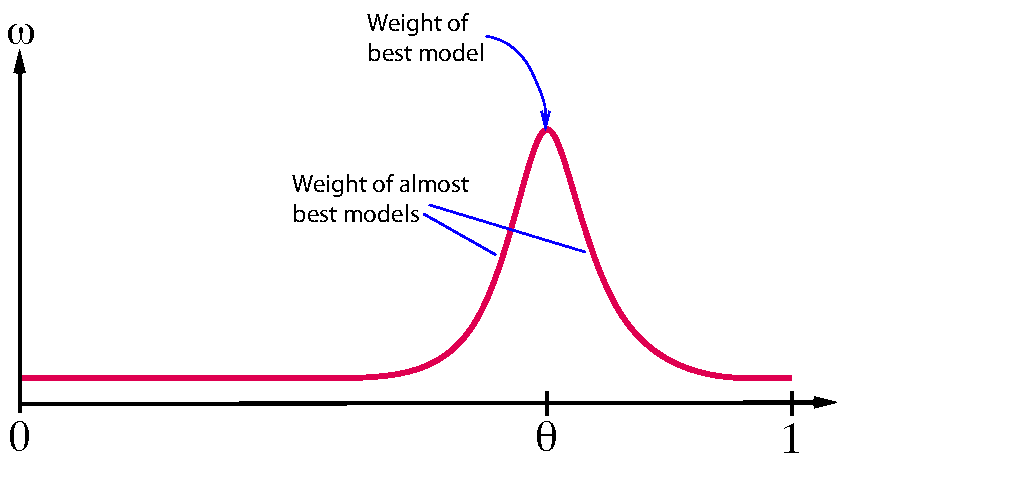
\includegraphics[height=6cm]{figures/neighborhood.pdf}
\end{frame}

%\subsection{Laplace Approximation}
\begin{frame}
\frametitle{Expanding the exponent around the peak}

\begin{itemize}
\item
For log loss the best \R{$\theta$} is empirical distribution
of the seq.
\R{\[
	\btheta = {\#\{x^t=1;\;\; 1 \leq t \leq T \} \over T} 
\]}
\item
The total loss scales with \R{$T$}
\R{\[
\TEloss{\theta} =
 T \cdot (\btheta \ell(\theta,1) + (1-\btheta)\ell(\theta,0))
 \doteq T \cdot g(\btheta,\theta)
\]}
\end{itemize}
\pause
\R{ \begin{eqnarray*}
\TAloss - \BEloss &\leq&
\ln \int_0^1 \dweight{\theta}{} e^{- \TEloss{\theta}} d\theta
- \ln e^{\BEloss} \\
\pause &=&
\ln \int_0^1 \dweight{\theta}{} e^{-
(\TEloss{\theta}-\BEloss)} d\theta \\
\pause &=&
\ln \int_0^1 \dweight{\theta}{} 
e^{T (g(\btheta,\theta) - g(\btheta,\btheta))} d\theta
\end{eqnarray*}}
\end{frame}

\begin{frame}
\frametitle{Laplace approximation (idea)}
\begin{itemize}
\item Taylor expansion of \R{$g(\btheta,\theta)-g(\btheta,\btheta)$} around \R{$\theta=\btheta$}.
\item
First and second terms in the expansion are zero.
\item
Third term gives a quadratic expression in the exponent
\item
$\Rightarrow$ a gaussian approximation of the posterior.
\end{itemize}
\pause
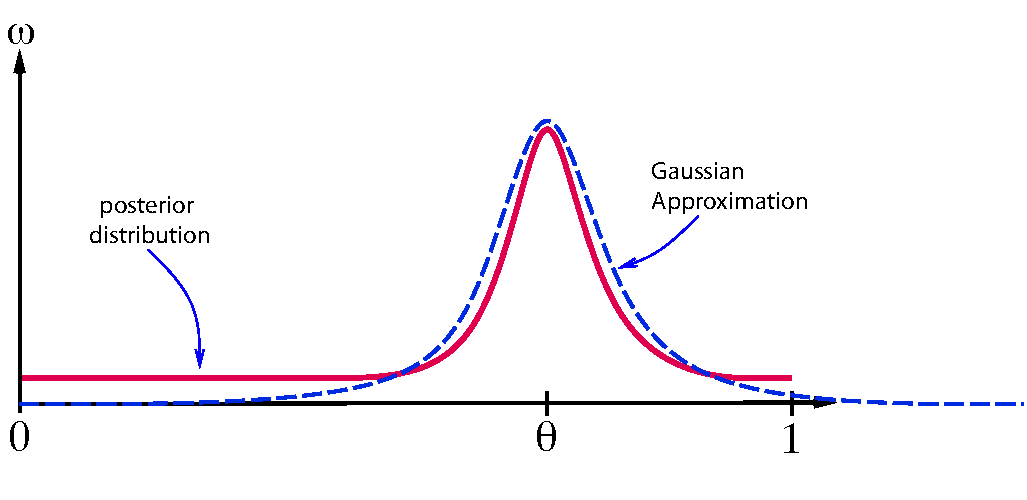
\includegraphics[height=5cm]{figures/Laplace.pdf}

\end{frame}

\begin{frame}
\frametitle{Laplace Approximation (details)}

\R{\begin{eqnarray*}
\lefteqn{\int_0^1  \dweight{\theta}{} 
         e^{T (g(\btheta,\theta)-g(\btheta,\btheta))} d\theta}\\
\pause &=& \dweight{\btheta}{} \sqrt{-2 \pi \over 
T \left. {d^2 \over d\theta^2} \right|_{\theta=\btheta} 
(g(\btheta,\theta)-g(\btheta,\btheta))}
+ O(T^{-3/2})
\end{eqnarray*}}
\end{frame}

%\subsection{Choosing the optimal prior}

\begin{frame}
\frametitle{Choosing the optimal prior}
\begin{itemize}
\item
Choose \R{$\dweight{\theta}{}$} to maximize the worst-case final total weight
\R{\[
\min_{\btheta} \dweight{\btheta}{} \sqrt{-2 \pi \over 
T \left. {d^2 \over d\theta^2} \right|_{\theta=\btheta} 
(g(\btheta,\theta)-g(\btheta,\btheta))}
\]}
\item
Make bound equal for all \R{$\btheta \in [0,1]$} by choosing
\R{\[
\dweight{\btheta}{*} =
{1 \over Z}
\sqrt{\left. {d^2 \over d\theta^2} \right|_{\theta=\btheta} 
(g(\btheta,\theta)-g(\btheta,\btheta)) \over - 2 \pi}~,
\]}
where \R{$Z$} is the normalization factor:
\R{\[
Z =\sqrt{1 \over 2 \pi}\;\;
\int_0^1 \;\;\sqrt{\left. {d^2 \over d\theta^2} \right|_{\theta=\btheta} 
(g(\btheta,\btheta)-g(\btheta,\theta))} \;\;d\btheta
\]}
\end{itemize}
\end{frame}


\begin{frame}
\frametitle{The bound for the optimal prior}
\begin{itemize}
\item Plugging in we get
\R{\begin{eqnarray*}
\TAloss - \BEloss &\leq&
\ln \int_0^1 \dweight{\theta}{*} 
e^{T (g(\btheta,\theta) - g(\btheta,\btheta))} d\theta \\
&=&
\ln \left( \sqrt{2\pi Z \over T} + O(T^{-3/2}) \right) \\
&=&
{1 \over 2} \ln {T \over 2\pi} -{1 \over 2} \ln Z + O(1/T)~.
\end{eqnarray*}}
\end{itemize}
\end{frame}

\begin{frame}
\frametitle{Solving for log-loss}
\begin{itemize}
\item
The exponent in the integral is
\R{\[
g(\btheta,\theta) - g(\btheta,\btheta)
=
\btheta \ln {\btheta \over \theta} + 
(1-\btheta) \ln {1-\btheta \over 1-\theta}
=
D_{KL} (\btheta || \theta)
\]}
\item
The second derivative
\R{\[
\left. {d^2 \over d\theta^2} \right|_{\theta=\btheta} 
D_{KL} (\btheta || \theta) = \btheta (1-\btheta)
\]}
Is called the \B{empirical Fisher information}
\item
The optimal prior:
\R{\[
\dweight{\btheta}{*} = \frac{1}{\pi \sqrt{\btheta (1-\btheta)}}
\]}
Known in general as \B{Jeffrey's prior}.  And, in this case, 
the \B{Dirichlet-$(1/2,1/2)$ prior}.
\end{itemize}
\end{frame}

\begin{frame}
\frametitle{The cumulative log loss of Bayes using Jeffrey's prior}
\begin{itemize}
\item
\R{\[
\TAloss - \BEloss \leq {1 \over 2} \ln (T+1) 
                     + {1 \over 2} \ln {\pi \over 2}
                     + O(1/T)
\]}
\end{itemize}
\end{frame}

%\subsection{Kritchevski Trofimov Prediction Rule}
\begin{frame}
\frametitle{But what is the prediction rule?}
\begin{itemize}
\item As luck would have it the Dirichlet prior is the \B{conjugate prior} for the Binomial distribution.
\item
Observed \R{$t$} bits, \R{$n$} of which were \R{$1$}. The posterior is:
\R{\[
\frac{1}{Z \sqrt{\theta(1-\theta)}} \theta^n (1-\theta)^{t-n} 
 = 
\frac{1}{Z} \theta^{n-1/2} (1-\theta)^{t-n-1/2} 
\]}
\item
The posterior average is:
\R{\[
\frac{\int_0^1 \theta^{n+1/2} (1-\theta)^{t-n-1/2} d\theta}
{\int_0^1 \theta^{n-1/2} (1-\theta)^{t-n-1/2} d\theta}
=
\frac{n+1/2}{t+1}
\]}
\item This is called the Trichevsky Trofimov prediction rule.
\end{itemize}
\end{frame}

%\subsection{Laplace Rule of Succession}
\begin{frame}
\frametitle{Laplace Rule of Succession}
\begin{itemize}
\item
Laplace suggested using the uniform prior, which is also a conjugate prior.
\item In this case the posterior average is:
\R{\[
\frac{\int_0^1 \theta^{n+1} (1-\theta)^{t-n} d\theta}
{\int_0^1 \theta^{n} (1-\theta)^{t-n} d\theta}
=
\frac{n+1}{t+2}
\]}
\item
The bound on the cumulative log loss is worse:
\R{\[
\TAloss - \BEloss = \ln T + O(1)
\]}
\item
Suffers larger regret when \R{$\btheta$} is far from \R{$1/2$}
\end{itemize}
\end{frame}

%\section{Priors for finite $t$}

%\section{Shtarkov lower bound for finite horizon}

\begin{frame}
\frametitle{Shtarkov Lower bound}
\begin{itemize}
\item What is the \B{optimal} prediction when \R{$T$} is know in
  advance?
\item
\R{\[
L_*^T - \min_\theta L_\theta^T \geq \frac{1}{2} \ln(T+1) + \frac{1}{2}
\ln \frac{\pi}{2} - O(\frac{1}{\sqrt{T}})
\]}
\end{itemize}
\end{frame}

\section{Generalization to larger sets of distributions}

\begin{frame}
\frametitle{Multinomial Distributions}
\begin{itemize}
\item For a distribution over \R{$k$} elements (Multinomial) \B{[Xie and Barron]}
\item Use the add 1/2 rule (KT).
\R{\[
p(i) = \frac{n_i+1/2}{t+k/2}
\]}
\item Bound is
\R{\[\TAloss - \BEloss \leq \frac{k-1}{2}\ln T + C + o(1)\]}
\item 
The constant C is optimal.
\end{itemize}
\end{frame}

\begin{frame}
\frametitle{Exponential Distributions}
\begin{itemize}
\item For any set of distributions from the exponential family
  defined by \R{$k$} parameters (constituting an open set) \B{[Rissanen96]}
\item Use Bayes Algorithm with Jeffrey's prior:
\R{\[
\dweight{\btheta}{*} = \frac{1}{Z} 
\frac{1}{\sqrt{
\left| \left. {\mathbf H} \paren{D_{KL} (\btheta || \theta) } \right|_{\theta=\btheta} \right|
}}
\]}
\R{$\mathbf H$} denotes the Hessian.
\item
\R{\[\TAloss - \BEloss \leq \frac{k-1}{2}\ln T - \ln Z + o(1)\]}
\end{itemize}
\end{frame}

\end{document}


\iffalse
\item {\bf 
\item Algorithm \R{$A$} predicts a sequence \R{$c^1,c^2,\ldots, c^T$}
over alphabet \R{$\Sigma = \{1,2,\ldots,k\}$}
\item The prediction for the \R{$c^t$}th is a distribution over \R{$\Sigma$}:\\
\R{$\vp_A^t = \langle p_A^t(1),p_A^t(2),\ldots,p_A^t(k) \rangle$} 
\item When $c^t$ is revealed, the loss we suffer is \R{$-\log p_A^t(c^t)$}
\item The {\color{blue}cumulative log loss}, which we wish to minimize, 
is \R{$\lossalg^T = -\sum_{t=1}^T \log p_A^t(c^t)$}
\item \R{$\lceil \lossalg^T \rceil$} is the code length if \R{$A$} is combined with arithmetic coding.
\end{itemize}
\end{frame}
\fi



